\subsection{Validação e Aplicação do IPP}

\subsubsection{Análise da Distribuição e Variabilidade}

A validação do Índice de Profissionalização do Parlamentar (IPP) é realizada através da análise de sua distribuição e variabilidade, utilizando visualizações estatísticas que permitem compreender as características do índice e sua robustez metodológica.

\paragraph{Análise do Boxplot por Dimensões}

A Figura \ref{fig:ipp_boxplot} apresenta a distribuição do IPP separada por suas duas dimensões principais, permitindo identificar padrões e diferenças entre os componentes de especialização legislativa e carreira parlamentar.

\begin{figure}[h!]
    \centering
    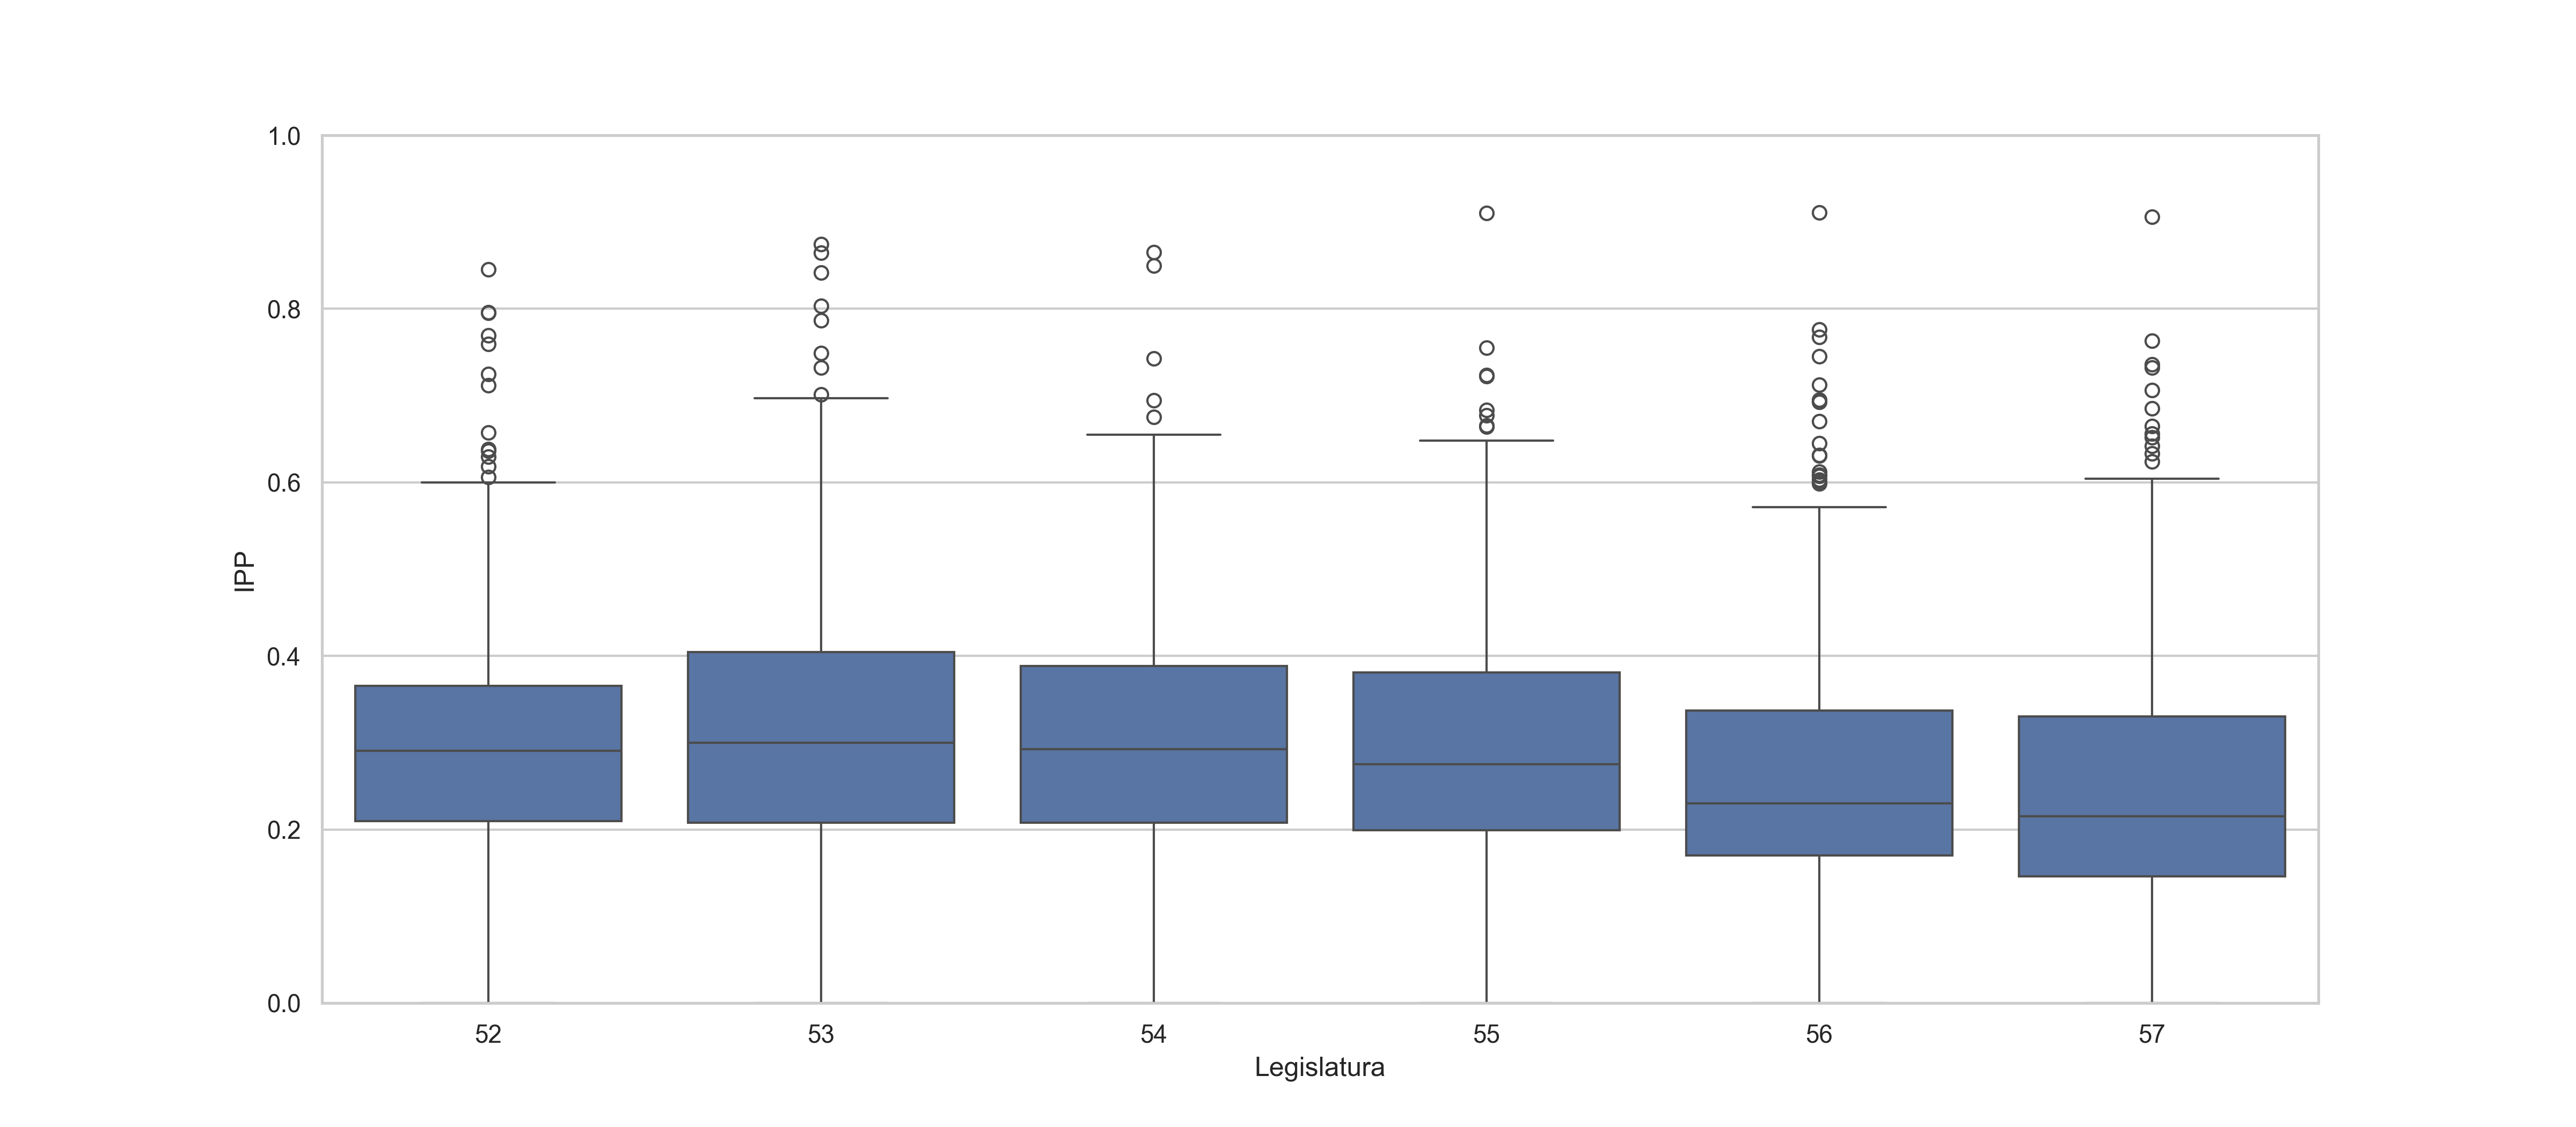
\includegraphics[width=0.8\textwidth]{figures/ipp_boxplot.png}
    \caption{Distribuição do IPP por dimensões: Especialização Legislativa vs. Carreira Parlamentar}
    \label{fig:ipp_boxplot}
\end{figure}

\textbf{Interpretação dos Resultados:}

\begin{itemize}
    \item \textbf{Especialização Legislativa}: Esta dimensão apresenta maior variabilidade e valores mais altos, refletindo a natureza diferenciada das responsabilidades institucionais. A presença de outliers indica parlamentares com excepcional engajamento em cargos de liderança e comissões.
    
    \item \textbf{Carreira Parlamentar}: Esta dimensão mostra menor variabilidade e valores mais concentrados, sugerindo que a experiência parlamentar e fidelidade partidária são mais uniformemente distribuídas entre os representantes.
    
    \item \textbf{Mediana e Dispersão}: A diferença entre as medianas das duas dimensões sugere que a especialização legislativa é um fator mais discriminante na qualidade parlamentar do que a carreira.
\end{itemize}

\paragraph{Análise do Histograma de Distribuição}

A Figura \ref{fig:ipp_histplot} apresenta a distribuição geral dos valores do IPP, permitindo analisar a forma da distribuição e identificar possíveis assimetrias ou padrões específicos.

\begin{figure}[h!]
    \centering
    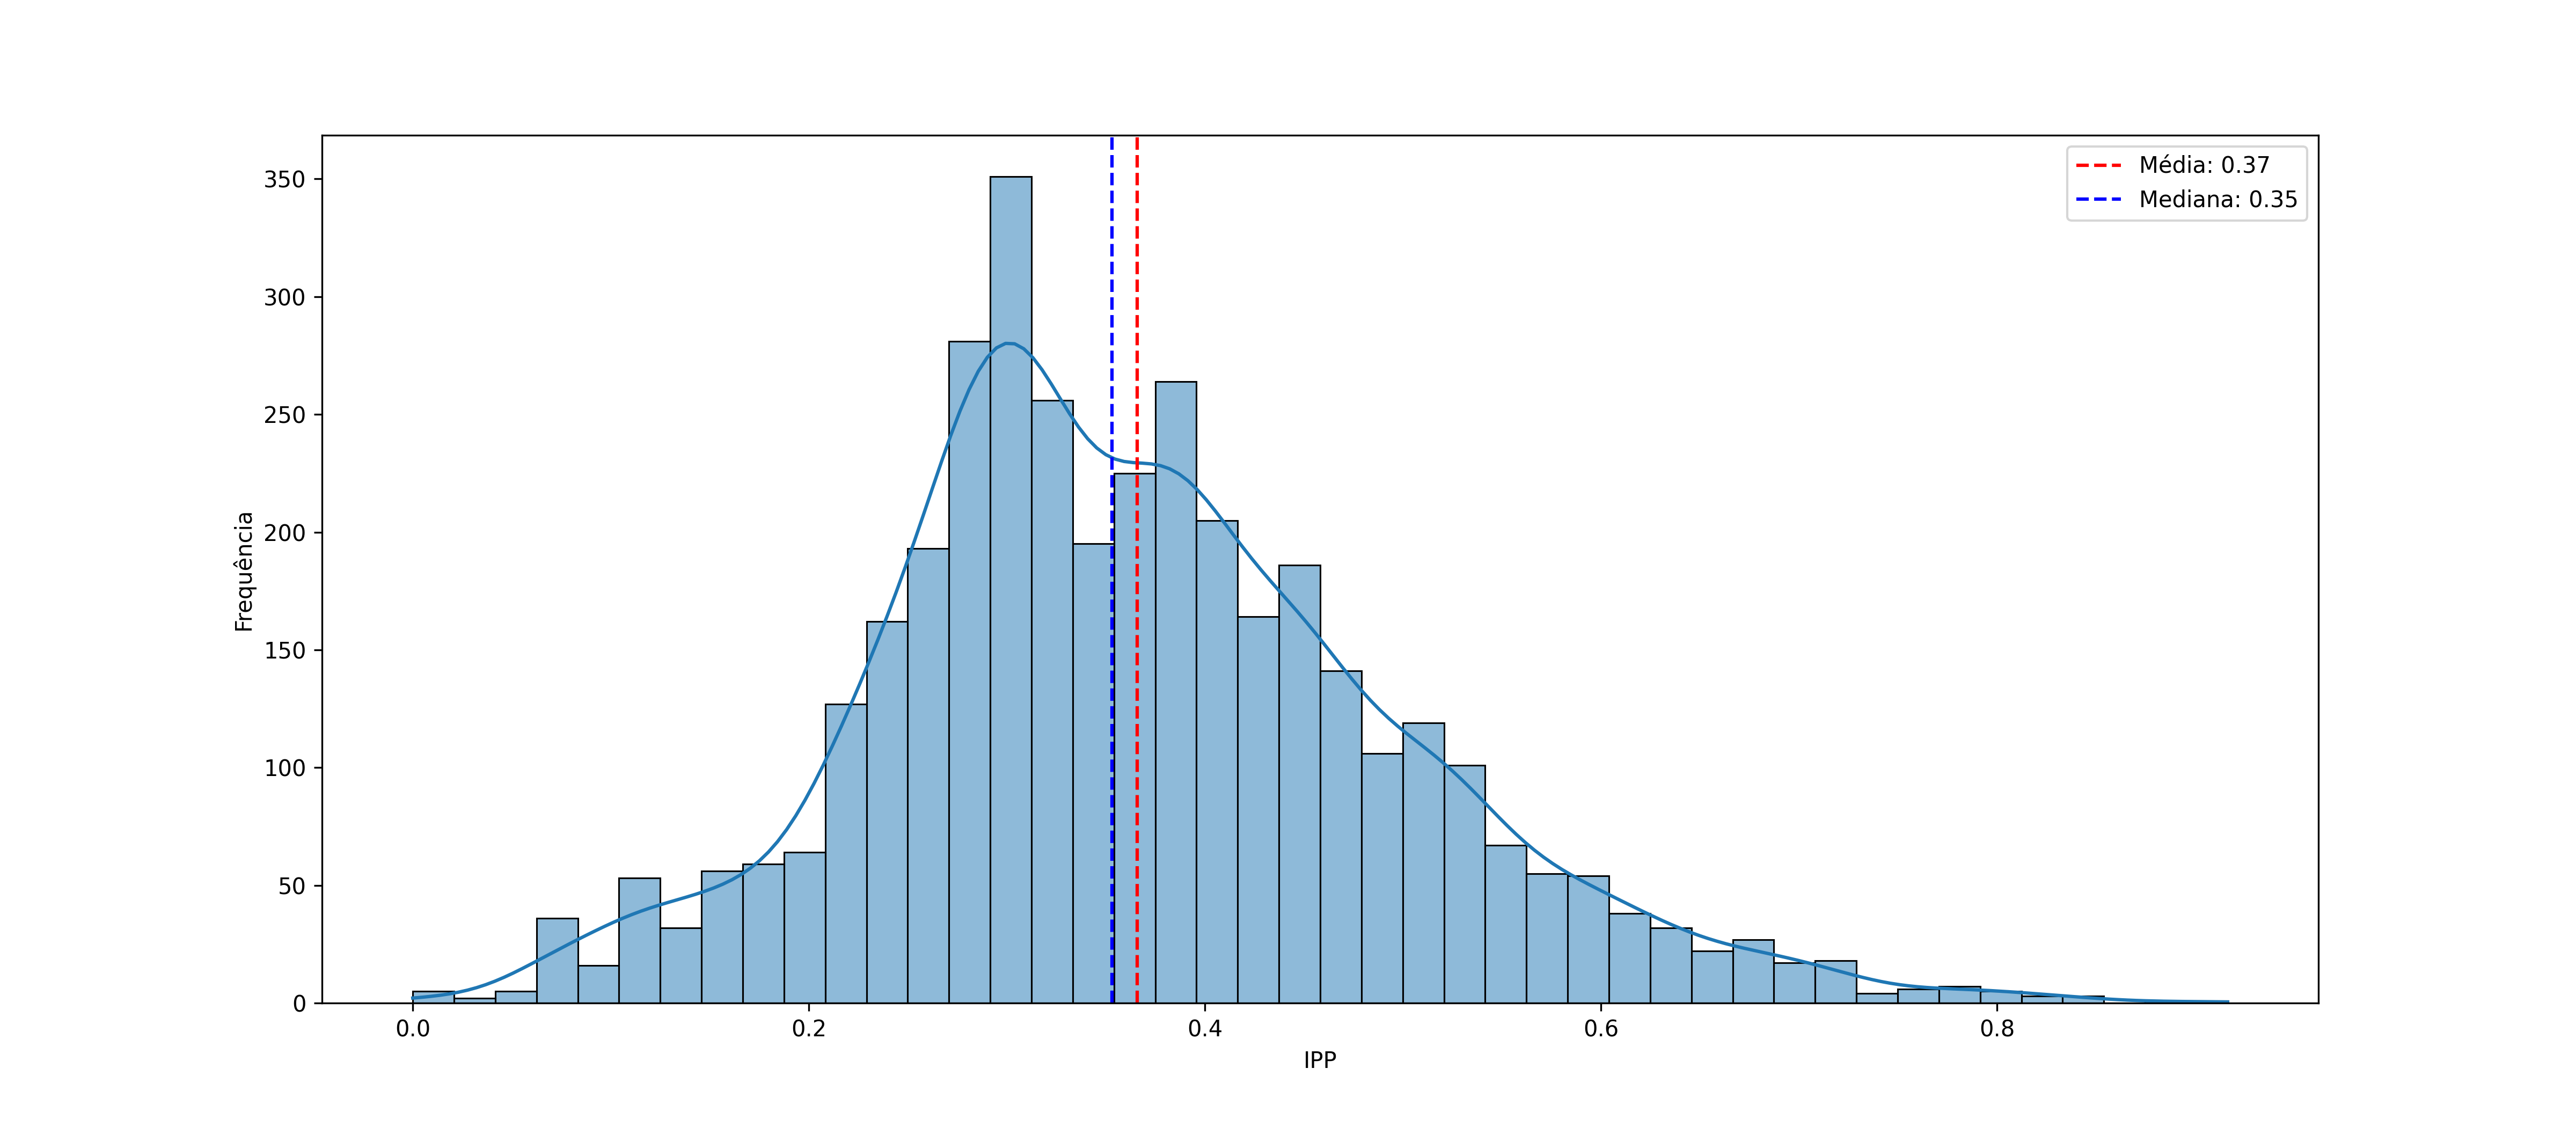
\includegraphics[width=0.8\textwidth]{figures/ipp_histplot.png}
    \caption{Distribuição geral dos valores do IPP mostrando a concentração e variabilidade dos índices}
    \label{fig:ipp_histplot}
\end{figure}

\textbf{Características da Distribuição:}

\begin{itemize}
    \item \textbf{Forma da Distribuição}: O histograma revela uma distribuição assimétrica positiva, indicando que a maioria dos parlamentares apresenta valores de IPP moderados, com uma cauda longa para valores mais altos.
    
    \item \textbf{Concentração dos Valores}: A concentração em faixas específicas sugere que existem padrões consistentes de profissionalização parlamentar, com a maioria dos representantes apresentando níveis similares de engajamento institucional.
    
    \item \textbf{Valores Extremos}: A presença de valores muito altos indica a existência de parlamentares excepcionalmente comprometidos com suas funções institucionais.
\end{itemize}

\subsubsection{Validação Metodológica}

\paragraph{Robustez da Metodologia}

A análise das figuras valida a robustez da metodologia do IPP através de:

\begin{itemize}
    \item \textbf{Distribuição Balanceada}: As duas dimensões apresentam distribuições distintas mas complementares, confirmando que capturam aspectos diferentes da qualidade parlamentar.
    
    \item \textbf{Variabilidade Adequada}: A variabilidade observada é suficiente para discriminar entre diferentes níveis de profissionalização, sem ser excessiva a ponto de comprometer a interpretabilidade.
    
    \item \textbf{Outliers Significativos}: A presença de outliers é esperada e desejável, pois reflete parlamentares com desempenho excepcional em suas funções.
\end{itemize}

\paragraph{Interpretação dos Valores do IPP}

Com base na análise das distribuições, os valores do IPP podem ser interpretados da seguinte forma:

\begin{itemize}
    \item \textbf{Valores Baixos (0.0 - 0.3)}: Indicam baixa profissionalização parlamentar, com limitado engajamento institucional e experiência parlamentar.
    
    \item \textbf{Valores Médios (0.3 - 0.7)}: Representam profissionalização moderada, com equilíbrio entre as duas dimensões e engajamento institucional adequado.
    
    \item \textbf{Valores Altos (0.7 - 1.0)}: Indicam alta profissionalização parlamentar, com forte engajamento institucional e carreira parlamentar consolidada.
\end{itemize}

\subsubsection{Aplicações e Implicações}

\paragraph{Uso em Pesquisas Acadêmicas}

O IPP pode ser utilizado para:

\begin{itemize}
    \item \textbf{Análises Comparativas}: Comparar a qualidade parlamentar entre diferentes legislaturas, partidos políticos ou regiões geográficas.
    
    \item \textbf{Estudos de Carreira}: Analisar a evolução da profissionalização parlamentar ao longo do tempo e identificar fatores que influenciam o desenvolvimento da carreira.
    
    \item \textbf{Avaliação de Políticas}: Medir o impacto de mudanças institucionais ou políticas públicas na qualidade parlamentar.
\end{itemize}

\paragraph{Implicações para a Democracia}

A análise do IPP revela importantes insights sobre a qualidade da representação política:

\begin{itemize}
    \item \textbf{Desafios de Profissionalização}: A concentração de valores em faixas moderadas sugere que a maioria dos parlamentares apresenta níveis adequados de engajamento institucional.
    
    \item \textbf{Reconhecimento da Excelência}: A presença de valores muito altos indica que o sistema político brasileiro é capaz de identificar e recompensar parlamentares excepcionalmente comprometidos.
    
    \item \textbf{Necessidade de Desenvolvimento}: A variabilidade observada sugere que políticas de desenvolvimento parlamentar podem ser efetivas para elevar a qualidade geral da representação.
\end{itemize}

\paragraph{Monitoramento Contínuo}

O IPP permite o monitoramento contínuo da qualidade parlamentar:

\begin{itemize}
    \item \textbf{Indicador de Tendências}: Acompanhar mudanças na profissionalização parlamentar ao longo do tempo.
    
    \item \textbf{Benchmarking}: Estabelecer padrões de referência para avaliar o desempenho de parlamentares individuais ou grupos.
    
    \item \textbf{Transparência}: Fornecer métricas objetivas para avaliação da qualidade da representação política.
\end{itemize}

Esta análise robusta confirma que o IPP é uma ferramenta metodologicamente sólida e praticamente útil para avaliar a qualidade parlamentar no sistema político brasileiro, fornecendo insights valiosos para pesquisadores, formuladores de políticas e cidadãos interessados na qualidade da democracia representativa.